% Boundra execution evidence report. Compile with Tectonic: tectonic -X compile execution-evidence.tex
\documentclass[11pt,a4paper,oneside]{report}
% Shared Boundra document style: fonts, brand colours, headings, callouts, tables, diagrams.
% Used by boundra-technical.tex, security-assessment.tex and execution-evidence.tex.

% ---------------------------------------------------------------- Page and fonts
\usepackage[a4paper,left=2.3cm,right=2.3cm,top=2.6cm,bottom=2.4cm,headheight=14pt]{geometry}
\usepackage{fontspec}
\setmainfont{Inter}[Extension=.otf,UprightFont=*-Regular,BoldFont=*-SemiBold,
  ItalicFont=*-Italic,BoldItalicFont=*-SemiBoldItalic,Scale=0.92]
\newfontfamily\headfont{SourceSerifPro}[Extension=.otf,UprightFont=*-Semibold,
  BoldFont=*-Bold,ItalicFont=*-SemiboldIt]
\setmonofont{SourceCodePro}[Extension=.otf,UprightFont=*-Regular,BoldFont=*-Semibold,Scale=0.86]
\linespread{1.12}
\setlength{\parindent}{0pt}
\setlength{\parskip}{0.55em}
\usepackage{microtype}
\usepackage{placeins}
\setlength{\emergencystretch}{3em}

% ---------------------------------------------------------------- Brand colours (apps/web/src/app/globals.css)
\usepackage{xcolor}
\definecolor{bForest}{HTML}{122D27}
\definecolor{bGreen}{HTML}{23674E}
\definecolor{bIvory}{HTML}{F6F8F2}
\definecolor{bSage}{HTML}{9BAF8D}
\definecolor{bLime}{HTML}{A6C74C}
\definecolor{bAmber}{HTML}{D8A13B}
\definecolor{bCharcoal}{HTML}{19332D}
\definecolor{bMuted}{HTML}{4D6058}
\definecolor{bMutedDark}{HTML}{B8C7BB}
\definecolor{bSurface}{HTML}{FCFDF9}
\definecolor{bSageSoft}{HTML}{E4EBDA}
\definecolor{bLimeSoft}{HTML}{E1ECBF}
\definecolor{bAmberSoft}{HTML}{F7E9CB}
\definecolor{bAmberInk}{HTML}{8A5A0B}
\definecolor{bLine}{HTML}{D3D9D2}
\color{bForest}

% ---------------------------------------------------------------- Packages
\usepackage{tikz}
\usetikzlibrary{svg.path,positioning,arrows.meta,shapes.geometric,fit,backgrounds,calc,shadows}
\usepackage[most]{tcolorbox}
\usepackage{booktabs,tabularx,xltabular,array,colortbl,multirow}
\usepackage{enumitem}
\usepackage{titlesec,titletoc}
\usepackage{fancyhdr}
\usepackage{listings}
\usepackage{amsmath}
\usepackage[hidelinks]{hyperref}
\hypersetup{pdftitle={Boundra: Technical Document},pdfauthor={Boundra team},
  colorlinks=true,linkcolor=bGreen,urlcolor=bGreen}

% ---------------------------------------------------------------- Headings
\titleformat{\chapter}[display]
  {\headfont\color{bForest}}
  {\normalfont\small\bfseries\color{bGreen}\MakeUppercase{Chapter}~\thechapter}
  {4pt}
  {\Huge}
  [\vspace{4pt}{\color{bLime}\rule{2.2cm}{2.5pt}}]
\titlespacing*{\chapter}{0pt}{-12pt}{18pt}
% A heading always keeps a few lines of its section with it on the page.
\titleformat{\section}{\headfont\Large\color{bForest}}{\color{bGreen}\thesection}{0.7em}{}
\titlespacing*{\section}{0pt}{1.4em}{0.5em}
\titleformat{\subsection}{\headfont\large\color{bForest}}{\color{bGreen}\thesubsection}{0.6em}{}
\titlespacing*{\subsection}{0pt}{1.1em}{0.35em}
\titleformat{\paragraph}[runin]{\bfseries\color{bForest}}{}{}{}[.]
\titlespacing*{\paragraph}{0pt}{0.5em}{0.6em}
\setcounter{secnumdepth}{2}
\setcounter{tocdepth}{1}

% Table of contents
\titlecontents{chapter}[2.2em]{\addvspace{0.42em}\headfont}
  {\contentslabel[\color{bGreen}\thecontentslabel]{2.2em}}{}{\hfill\contentspage}
\titlecontents{section}[4.8em]{\small}
  {\contentslabel[\color{bMuted}\thecontentslabel]{2.6em}}{}
  {\titlerule*[0.6pc]{\color{bLine}.}\contentspage}

% ---------------------------------------------------------------- Header and footer
\pagestyle{fancy}
\fancyhf{}
\renewcommand{\chaptermark}[1]{\markboth{#1}{}}
% Each document sets its own name with \renewcommand{\docname}{...} after loading this style.
\newcommand{\docname}{Technical document}
\fancyhead[L]{\small\color{bMuted}\brandmark[0.17]\hspace{0.45em}Boundra\,·\,\docname}
\fancyhead[R]{\small\color{bMuted}\nouppercase{\leftmark}}
\fancyfoot[R]{\small\color{bGreen}\bfseries\thepage}
\fancyfoot[L]{\small\color{bMuted}Base Sepolia testnet prototype\,·\,no real funds}
\renewcommand{\headrule}{{\color{bLine}\hrule height 0.5pt}}
\fancypagestyle{plain}{\fancyhf{}\renewcommand{\headrule}{}
  \fancyfoot[R]{\small\color{bGreen}\bfseries\thepage}}

% ---------------------------------------------------------------- Lists
\setlist{itemsep=0.15em,topsep=0.25em,parsep=0.1em}
\setlist[itemize,1]{label={\color{bLime}\rule[0.18em]{0.42em}{0.42em}},leftmargin=1.3em}
\setlist[itemize,2]{label={\color{bSage}\textbullet},leftmargin=1.2em}
\setlist[enumerate,1]{label={\color{bGreen}\bfseries\arabic*.},leftmargin=1.6em}

% ---------------------------------------------------------------- Brand mark (apps/web/src/components/brand-mark.tsx)
\newcommand{\markforest}{svg{M9.4 9.7C8.6 10.5 7.3 12 6.3 13.2C5.4 14.5 4.6 15.9 3.8 17.2C3.1 18.5 2.4 19.8 1.9 21.2C1.3 22.6 0.9 24.1 0.5 25.6C0.2 27.1 0.1 28.6 0 30.1C-0.1 31.6 0 33.2 0.2 34.7C0.4 36.2 0.7 37.8 1.1 39.2C1.5 40.7 2 42.1 2.7 43.5C3.3 44.9 4 46.3 4.8 47.6C5.6 48.8 6.5 50.1 7.5 51.2C8.5 52.4 9.6 53.5 10.8 54.4C11.9 55.4 13.1 56.3 14.4 57.2C15.6 58 16.9 58.7 18.3 59.3C19.6 59.9 21 60.5 22.4 60.9C23.8 61.4 25.3 61.8 26.9 62C28.4 62.2 30.1 62.4 31.6 62.3C33.2 62.2 34.9 61.9 36.3 61.4C37.8 61 39.2 60.4 40.5 59.8C41.8 59.1 43.1 58.4 44.2 57.6C45.3 56.8 46.4 55.9 47.4 55C48.4 54.1 49.3 53.1 50.1 52.1C51 51.1 51.8 50 52.3 49.2C52.8 48.4 53.2 47.9 53.3 47.2C53.5 46.5 53.4 45.6 53.2 44.9C53 44.2 52.5 43.5 51.9 43C51.4 42.5 50.6 42.2 49.9 42C49.2 41.9 48.3 41.9 47.6 42.2C47 42.4 46.4 42.8 45.8 43.4C45.1 44 44.3 44.9 43.6 45.5C42.8 46.1 42 46.5 41.3 47C40.5 47.4 39.6 47.8 38.8 48.1C38 48.4 37.1 48.7 36.3 48.9C35.4 49.1 34.6 49.3 33.8 49.3C33 49.4 32.3 49.4 31.5 49.3C30.8 49.2 30 49.1 29.3 48.9C28.5 48.7 27.7 48.4 27 48.1C26.2 47.8 25.4 47.4 24.7 46.9C23.9 46.5 23.2 46 22.6 45.5C21.9 44.9 21.3 44.4 20.8 43.8C20.2 43.2 19.7 42.5 19.2 41.9C18.8 41.2 18.4 40.5 18 39.8C17.6 39 17.3 38.3 17 37.5C16.7 36.7 16.4 35.9 16.2 35.1C16 34.3 15.9 33.5 15.7 32.7C15.6 31.8 15.5 31 15.5 30.1C15.4 29.2 15.4 28.3 15.4 27.3C15.4 26.4 15.3 25.5 15.3 24.4C15.4 23.4 15.6 22.3 15.7 21.1C15.7 20 15.6 18.7 15.8 17.5C16 16.2 16.5 14.7 16.7 13.7C17 12.7 17.3 12.3 17.3 11.6C17.2 10.9 17 10.1 16.6 9.5C16.3 8.9 15.7 8.4 15.1 8C14.5 7.7 13.7 7.5 13 7.5C12.3 7.5 11.5 7.8 10.9 8.1C10.3 8.5 10.2 8.8 9.4 9.7Z}}
\newcommand{\marksage}{svg{M26.2 9.5C26.9 9.5 27.8 9.3 28.5 9.2C29.2 9.1 29.9 9.1 30.6 9.1C31.3 9.2 32 9.2 32.7 9.3C33.4 9.4 34 9.5 34.7 9.7C35.4 9.8 36 10 36.7 10.2C37.3 10.4 38 10.6 38.6 10.9C39.2 11.1 39.9 11.4 40.5 11.7C41.1 12 41.7 12.3 42.2 12.6C42.8 13 43.4 13.3 43.9 13.7C44.4 14.1 45 14.5 45.5 14.9C46 15.4 46.5 15.8 46.9 16.3C47.4 16.7 47.8 17.2 48.3 17.7C48.7 18.2 49.1 18.7 49.5 19.3C49.9 19.8 50.2 20.3 50.6 20.9C50.9 21.4 51.3 22 51.6 22.6C51.9 23.1 52.2 23.7 52.5 24.3C52.8 24.9 53.1 25.6 53.3 26.2C53.5 26.8 53.8 27.5 54 28.1C54.1 28.8 54.3 29.4 54.4 30.1C54.6 30.8 54.7 31.5 54.7 32.2C54.8 32.9 54.8 33.5 54.8 34.3C54.7 35 54.6 35.8 54.6 36.5C54.6 37.2 54.5 37.9 54.8 38.5C55 39.1 55.4 39.7 55.9 40.1C56.4 40.5 57.1 40.8 57.7 40.9C58.4 41 59.1 40.9 59.7 40.7C60.3 40.4 60.9 40 61.3 39.5C61.7 39 61.8 38.4 62.1 37.7C62.3 37 62.4 36 62.6 35.1C62.7 34.2 62.9 33.3 63 32.3C63.1 31.4 63.1 30.5 63.1 29.5C63.1 28.6 63.1 27.6 63 26.6C63 25.7 62.9 24.7 62.7 23.8C62.5 22.8 62.3 21.8 62 20.9C61.8 20 61.4 19 61.1 18.1C60.7 17.2 60.3 16.3 59.8 15.5C59.3 14.6 58.8 13.8 58.2 13C57.6 12.2 57 11.4 56.3 10.6C55.7 9.9 55 9.2 54.3 8.5C53.5 7.9 52.8 7.2 52 6.7C51.2 6.1 50.4 5.5 49.5 5C48.7 4.5 47.8 4 47 3.6C46.1 3.2 45.2 2.8 44.3 2.5C43.4 2.1 42.4 1.8 41.5 1.6C40.6 1.3 39.6 1.1 38.7 1C37.7 0.9 36.7 0.8 35.8 0.7C34.8 0.7 33.9 0.7 32.9 0.7C32 0.8 31 0.9 30.1 1C29.1 1.1 28.2 1.3 27.3 1.4C26.4 1.6 25.4 1.8 24.7 2.1C24 2.3 23.4 2.5 23 3C22.5 3.4 22.1 4 21.9 4.6C21.7 5.2 21.6 5.9 21.7 6.6C21.9 7.2 22.2 7.8 22.6 8.3C23 8.8 23.7 9.2 24.3 9.4C24.9 9.6 25.5 9.6 26.2 9.5Z}}
% \brandmarkcol[scale]{outer colour}: the mark on its 64-unit grid (1 unit = 1pt at scale 1),
% with the forest arc in the given colour. \brandmark[scale] is the light-surface version.
\newcommand{\brandmarkcol}[2][1]{\begin{tikzpicture}[scale=#1,yscale=-1,
  baseline={([yshift=-1.2pt]current bounding box.south)}]
  \fill[#2] \markforest;
  \fill[bSage] \marksage;
  \fill[bLime] (32pt,32pt) circle (8.4pt);
\end{tikzpicture}}
\newcommand{\brandmark}[1][1]{\brandmarkcol[#1]{bForest}}

% ---------------------------------------------------------------- Callout boxes
\tcbset{boundra/.style={enhanced,boxrule=0pt,arc=3pt,left=10pt,right=10pt,
  top=7pt,bottom=7pt,fonttitle=\bfseries\small,coltitle=bForest,attach title to upper,
  before skip=0.9em,after skip=0.9em}}
\newtcolorbox{keypoint}[1][Key point]{boundra,colback=bLimeSoft,
  borderline west={3pt}{0pt}{bGreen},title={#1.\ }}
\newtcolorbox{note}[1][Note]{boundra,colback=bSageSoft,
  borderline west={3pt}{0pt}{bSage},title={#1.\ }}
\newtcolorbox{caution}[1][Caution]{boundra,colback=bAmberSoft,coltitle=bAmberInk,
  borderline west={3pt}{0pt}{bAmber},title={#1.\ }}
\newtcolorbox{principle}[1]{enhanced,boxrule=0pt,arc=4pt,colback=bForest,
  coltext=bIvory,left=12pt,right=12pt,top=9pt,bottom=9pt,fonttitle=\headfont\large,
  coltitle=bLime,title={#1},attach title to upper={\par\vspace{3pt}},before skip=1em,after skip=1em}

% ---------------------------------------------------------------- Tables
\newcolumntype{L}{>{\raggedright\arraybackslash}X}
\newcolumntype{P}[1]{>{\raggedright\arraybackslash}p{#1}}
\renewcommand{\arraystretch}{1.28}
\setlength{\tabcolsep}{5pt}
\arrayrulecolor{bSage}
\newcommand{\thead}[1]{\textbf{\color{bForest}#1}}
\newcommand{\headrow}{\rowcolor{bSageSoft}}
% Tables break across pages (xltabular = longtable + X columns) instead of leaving gaps.
\setlength{\LTleft}{0pt}
\setlength{\LTright}{0pt}
\setlength{\LTpre}{0pt}
\setlength{\LTpost}{0.4em}
% A table never starts on a new page away from the heading or text just above it.
\newenvironment{btable}[1]
  {\par\nopagebreak\vspace{0.6em}\small\xltabular{\linewidth}{#1}\toprule}
  {\bottomrule\endxltabular\par}
% Short tables (up to about eight rows) never split; they move with the heading or text above.
\newenvironment{stable}[1]
  {\par\nopagebreak\vspace{0.6em}\small\noindent\tabularx{\linewidth}{#1}\toprule}
  {\bottomrule\endtabularx\par\vspace{0.4em}}

% Floats: allow them close to their text, and top-align pages that hold only floats.
\renewcommand{\topfraction}{0.9}
\renewcommand{\bottomfraction}{0.8}
\renewcommand{\textfraction}{0.08}
\renewcommand{\floatpagefraction}{0.8}
\makeatletter
\setlength{\@fptop}{0pt}
\makeatother

% ---------------------------------------------------------------- Code and inline helpers
\lstdefinestyle{boundra}{basicstyle=\ttfamily\small\color{bForest},backgroundcolor=\color{bSurface},
  frame=single,rulecolor=\color{bLine},framesep=6pt,xleftmargin=6pt,xrightmargin=6pt,
  keywordstyle=\color{bGreen}\bfseries,commentstyle=\color{bMuted}\itshape,
  stringstyle=\color{bAmberInk},columns=fullflexible,keepspaces=true,breaklines=true,
  showstringspaces=false,aboveskip=0.8em,belowskip=0.6em}
\lstset{style=boundra}
\newcommand{\code}[1]{\texttt{\color{bGreen}#1}}
% Inside dark diagram boxes, code takes the box's text colour instead of green.
\newcommand{\plaincode}{\renewcommand{\code}[1]{\texttt{##1}}}
\newcommand{\term}[1]{\textbf{#1}}
\newcommand{\muted}[1]{{\color{bMuted}#1}}

% ---------------------------------------------------------------- Diagram styles
\tikzset{
  box/.style={draw=bForest,line width=0.6pt,rounded corners=3pt,fill=white,align=center,
    font=\small,inner sep=5pt,minimum height=9mm,text=bForest,
    execute at begin node={\hyphenpenalty=10000\exhyphenpenalty=10000}},
  % On dark fills, code takes the box's text colour instead of green.
  boxdark/.style={box,fill=bForest,text=bIvory,draw=bForest,
    execute at begin node={\hyphenpenalty=10000\exhyphenpenalty=10000\plaincode}},
  boxgreen/.style={box,fill=bGreen,text=white,draw=bGreen,
    execute at begin node={\hyphenpenalty=10000\exhyphenpenalty=10000\plaincode}},
  boxlime/.style={box,fill=bLimeSoft},
  boxsage/.style={box,fill=bSageSoft},
  boxamber/.style={box,fill=bAmberSoft,draw=bAmberInk},
  boxghost/.style={box,draw=bSage,dashed,text=bMuted},
  arr/.style={-{Stealth[length=2.2mm,width=1.8mm]},line width=0.65pt,draw=bGreen},
  arrm/.style={arr,draw=bMuted},
  arrd/.style={arr,dashed,draw=bMuted},
  arra/.style={arr,draw=bAmberInk},
  biarr/.style={{Stealth[length=2.2mm,width=1.8mm]}-{Stealth[length=2.2mm,width=1.8mm]},
    line width=0.65pt,draw=bGreen},
  lbl/.style={font=\scriptsize,text=bMuted,fill=white,inner sep=1.5pt,align=center},
  lblc/.style={font=\scriptsize,text=bMuted,inner sep=1.5pt,align=center},
  zone/.style={draw=bSage,line width=0.6pt,dashed,rounded corners=6pt,inner sep=9pt},
  zonefill/.style={fill=bSurface,draw=bSage,line width=0.6pt,rounded corners=6pt,inner sep=9pt},
  zonetitle/.style={font=\scriptsize\bfseries,text=bGreen,fill=white,inner sep=2pt},
  state/.style={draw=bForest,line width=0.6pt,rounded corners=7pt,fill=white,font=\scriptsize\ttfamily,
    inner sep=4pt,minimum height=7mm,text=bForest},
  stateok/.style={state,fill=bLimeSoft},
  statebad/.style={state,fill=bAmberSoft,draw=bAmberInk},
  statedone/.style={state,fill=bSageSoft},
  stepdot/.style={circle,fill=bGreen,text=white,font=\scriptsize\bfseries,inner sep=1.4pt,minimum size=4.6mm},
}
\newcommand{\stepno}[1]{\tikz[baseline=-0.6ex]\node[stepdot]{#1};}

\newcommand{\figcaption}[1]{\par\vspace{0.3em}{\centering\small\color{bMuted}#1\par}\vspace{0.6em}}


\renewcommand{\docname}{Execution evidence}
\hypersetup{pdftitle={Boundra: Execution Evidence}}
\renewcommand{\thesection}{\arabic{section}}
\renewcommand{\sectionmark}[1]{\markboth{#1}{}}
% \tx{full hash}{short label}: a Basescan link to one transaction.
\newcommand{\tx}[2]{\href{https://sepolia.basescan.org/tx/#1}{\texttt{\color{bGreen}#2}}}
\newcommand{\addr}[2]{\href{https://sepolia.basescan.org/address/#1}{\texttt{\color{bGreen}#2}}}
\newcommand{\fullhash}[1]{\href{https://sepolia.basescan.org/tx/#1}{\texttt{\fontsize{6}{7.5}\selectfont\color{bGreen}#1}}}

\begin{document}

\begin{titlepage}
\thispagestyle{empty}

\begin{tikzpicture}[remember picture,overlay]
  \fill[bForest] (current page.south west) rectangle (current page.north east);
  \draw[bGreen,line width=26pt,opacity=0.35]
    ($(current page.south east)+(-2.2,6.5)$) arc[start angle=-10,end angle=120,radius=9.5];
  \draw[bLime,line width=3pt,opacity=0.55]
    ($(current page.south east)+(-1.2,4.6)$) arc[start angle=-20,end angle=95,radius=7.2];
  \node[anchor=north west,inner sep=0] at ($(current page.north west)+(2.3,-2.6)$)
    {\brandmarkcol[1.5]{bIvory}};
  \node[anchor=north west,inner sep=0,text width=14.5cm,align=left]
    at ($(current page.north west)+(2.3,-6.4)$) {%
    {\color{bLime}\small\bfseries\MakeUppercase{Submission item 06}}\\[10pt]
    {\headfont\fontsize{40}{46}\selectfont\color{bIvory}\spaceskip=0.26em Execution evidence}\\[12pt]
    {\headfont\LARGE\color{bIvory}Real transactions on Base Sepolia}\\[18pt]
    {\large\color{bMutedDark}One owner journey on the deployed app: 16 transactions, each read\\[2pt]
      back from the chain, including the agent acting on its own.}};
  \node[anchor=south west,inner sep=0,text width=15cm,align=left]
    at ($(current page.south west)+(2.3,2.4)$) {%
    {\small\color{bMutedDark}%
    \begin{tabular}{@{}l@{\hspace{1.2em}}l@{}}
      \color{bLime}\bfseries Event   & FinTechathon 2026, Topic F (on-chain)\\
      \color{bLime}\bfseries Network & Base Sepolia testnet (chain 84532)\\
      \color{bLime}\bfseries App     & \texttt{https://boundra-api.onrender.com}\\
      \color{bLime}\bfseries Blocks  & 48,368,221 to 48,368,421, 20 October 2026\\
    \end{tabular}}};
\end{tikzpicture}
\end{titlepage}

\section{Summary}

An owner used the deployed Boundra app to give Boundra's agent a mandate: put 300 MockUSDC into LiquidVault, with withdrawals allowed at any time. The owner signed every authority and funding transaction in their own wallet; the agent then made the deposit by itself, with its own key; the owner paused, resumed, took the funds back and revoked the mandate. All 16 transactions succeeded on chain.

\begin{stable}{@{}P{3.6cm}L@{}}
\headrow \thead{Who} & \thead{Address}\\ \midrule
Owner & \addr{0xEcc070725898eb3aaea8448b16272eE6E56c5e81}{0xEcc070725898eb3aaea8448b16272eE6E56c5e81}\\
Owner's executor & \addr{0x0e4c01b7fAc2e45a2a38eA7B9A0744D4eF0e9E2E}{0x0e4c01b7fAc2e45a2a38eA7B9A0744D4eF0e9E2E}\\
Boundra's agent (operator) & \addr{0x7d8616836B3fC6FFABE090a4d3658e5a5C3A87F1}{0x7d8616836B3fC6FFABE090a4d3658e5a5C3A87F1}\\
Factory & \addr{0xFbD91368BfFA9AF5C7034bCB7F53Cc1eC906b7f4}{0xFbD91368BfFA9AF5C7034bCB7F53Cc1eC906b7f4}\\
LiquidVault & \addr{0x7C0fC1a0551d5099d093E8D8b34a214758f7B27a}{0x7C0fC1a0551d5099d093E8D8b34a214758f7B27a}\\
MockUSDC & \addr{0x13e7a4d02941a029Cf841f16E38eF377cb21e1Cf}{0x13e7a4d02941a029Cf841f16E38eF377cb21e1Cf}\\
\end{stable}

\begin{principle}{What the evidence shows}
The agent acted alone, with its own key, and only within the limits the owner signed; the owner kept every key and every control; funds only ever returned to the owner.
\end{principle}

\section{The journey}

\begin{figure}[htbp]
\centering
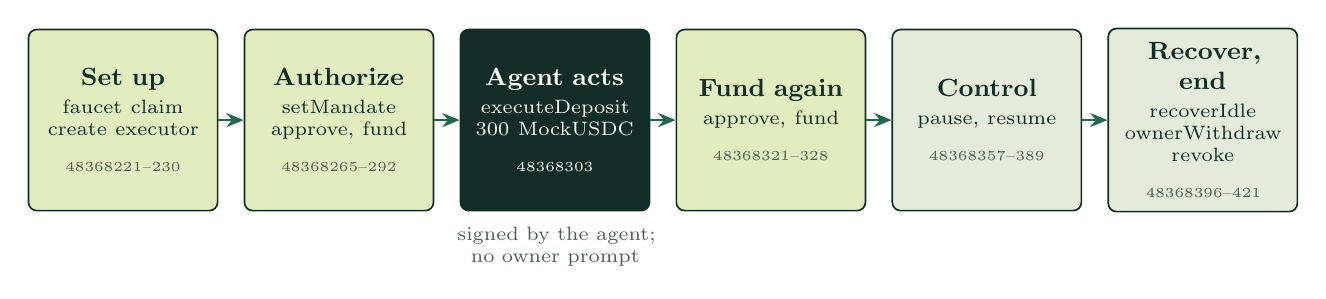
\begin{tikzpicture}[node distance=0.32cm]
  \node[boxlime,text width=2.05cm,minimum height=2.3cm] (p1) {\textbf{Set up}\\[2pt]\scriptsize faucet claim\\create executor\\[2pt]\muted{\tiny 48368221--230}};
  \node[boxlime,text width=2.05cm,minimum height=2.3cm,right=of p1] (p2) {\textbf{Authorize}\\[2pt]\scriptsize setMandate\\approve, fund\\[2pt]\muted{\tiny 48368265--292}};
  \node[boxdark,text width=2.05cm,minimum height=2.3cm,right=of p2] (p3) {\textbf{Agent acts}\\[2pt]\scriptsize executeDeposit\\300 MockUSDC\\[2pt]{\tiny 48368303}};
  \node[boxlime,text width=2.05cm,minimum height=2.3cm,right=of p3] (p4) {\textbf{Fund again}\\[2pt]\scriptsize approve, fund\\[2pt]\muted{\tiny 48368321--328}};
  \node[boxsage,text width=2.05cm,minimum height=2.3cm,right=of p4] (p5) {\textbf{Control}\\[2pt]\scriptsize pause, resume\\[2pt]\muted{\tiny 48368357--389}};
  \node[boxsage,text width=2.05cm,minimum height=2.3cm,right=of p5] (p6) {\textbf{Recover, end}\\[2pt]\scriptsize recoverIdle\\ownerWithdraw\\revoke\\[2pt]\muted{\tiny 48368396--421}};
  \foreach \a/\b in {1/2,2/3,3/4,4/5,5/6}{\draw[arr] (p\a) -- (p\b);}
  \node[lblc,below=4pt of p3,text width=3.4cm] {signed by the agent; no owner prompt};
\end{tikzpicture}
\caption{Owner transactions in light boxes, the agent's in the dark box. Block numbers below each phase.}
\end{figure}

\begin{keypoint}[The agent's own transaction]
Eleven blocks after the executor was funded, the worker proposed a deposit, checked it against the confirmed mandate, simulated it, signed it with the agent's key and sent it:
\tx{0xb9e053eb35b4780703d9d6e6e79f045d3401fb219afea3c6789471574740100b}{0xb9e053eb…0100b}, block 48,368,303, from the agent to the owner's executor, \code{executeDeposit} of 300 MockUSDC into LiquidVault, status success. The single allocation was then complete, so the agent held and sent nothing more.
\end{keypoint}

\newpage
\section{All transactions}

\begin{btable}{@{}P{1.7cm}P{1.2cm}P{4.2cm}L@{}}
\headrow \thead{Block} & \thead{Sender} & \thead{Call} & \thead{Transaction hash (Basescan)}\\ \midrule\endhead
48368221 & owner & Faucet \code{claim} & \fullhash{0x74f57e9df29dab05d4aab933cf296c8f5d5e32afb02cabda189c536464c04fc0}\\
48368230 & owner & Factory \code{createExecutor} & \fullhash{0x815efb6f67f5db80d164689e9ef13ce405d91fe9eab271f286b287b682a18808}\\
48368265 & owner & Executor \code{setMandate} & \fullhash{0xe648e4e4b2e0717c0fa014da53f87024cb78d7d05edb7543fb23579b3041797d}\\
48368283 & owner & MockUSDC \code{approve} & \fullhash{0x4f3609689d393939bad1eee1766d37abee5a4c0b75c5ac770bea1a7a4f453b0d}\\
48368292 & owner & Executor \code{fund} & \fullhash{0xf67668a01d46122526af2eafe582511e570ddf833fea7d3764269ff17c599300}\\
\rowcolor{bLimeSoft} 48368303 & \textbf{agent} & Executor \code{executeDeposit} & \fullhash{0xb9e053eb35b4780703d9d6e6e79f045d3401fb219afea3c6789471574740100b}\\
48368321 & owner & MockUSDC \code{approve} & \fullhash{0xe1704fcc1ea7919da1b3489af32237b76120c0063b6456343bfa4d2d59af9b05}\\
48368328 & owner & Executor \code{fund} & \fullhash{0x23e0c927b0fc41cbf3844d806769897c128f85f2265fa1183fd7ba48ee473151}\\
48368357 & owner & Executor \code{pause} & \fullhash{0xdfd3c2eff130eb00fbf0e8cb09b9b4ba7d95db840691d43d66e7d1e8133babc7}\\
48368373 & owner & Executor \code{pause} (repeat) & \fullhash{0xc0bd425776bd4bc5783cfd92c555d7e7f50ed3455ddf3de09c561c482458bb91}\\
48368382 & owner & Executor \code{resume} & \fullhash{0xb7251b4d5495e56506c26366718648689144019a1edb7cbfe8f0f28b6e7d1abe}\\
48368389 & owner & Executor \code{resume} (repeat) & \fullhash{0x2ab19ea34d287c9f8f242ddb2c79aff38d6010fabcbf05017a80e21b8e8ffdf5}\\
48368396 & owner & Executor \code{recoverIdle} & \fullhash{0x56efae44fc317b28e958f5e99e56743cbf553dd26f6b0999dd28e5a94117c564}\\
48368408 & owner & Executor \code{ownerWithdraw} & \fullhash{0xef7e0b9a59098e90d42fec06446533bc332715c9540953de96f4e32a1829d9e9}\\
48368417 & owner & Executor \code{revoke} & \fullhash{0x7dbd39a2384c624bd5fa784e40fb4b835f5097e423db27e739a111502699960c}\\
48368421 & owner & Executor \code{revoke} (repeat) & \fullhash{0xce1de1440d4084d9ffee8929a4f8a22f2e482320f02eed6b957bca5d0e958812}\\
\end{btable}

Every transaction above has status \textbf{success}. Senders and targets were read back from the chain: the owner's wallet signed every owner transaction, and only the agent's address signed the deposit.

\begin{note}[About the repeats]
Pause, resume and revoke appear twice because the app did not show the new state until the page was reloaded, so the owner sent them again. The first of each pair had already taken effect; both succeed on chain. A fix (the overview polls until the confirmed block and disables the controls meanwhile) is in pull request \#11.
\end{note}

\section{What it proves}

\begin{stable}{@{}P{4.4cm}L@{}}
\headrow \thead{Claim} & \thead{Evidence above}\\ \midrule
The owner keeps every key & Every owner transaction is signed by the owner's address; the server never signed for them.\\
The agent acts on its own & The deposit is signed by the agent's address, with no owner transaction in that block.\\
The agent stays within the mandate & The executor accepted \code{executeDeposit} only after \code{setMandate} and \code{fund}; it sent nothing after the single allocation.\\
The owner stays in control & \code{pause} and \code{resume} stopped and restarted the agent; \code{revoke} ended the mandate for good.\\
Funds return only to the owner & \code{recoverIdle} and \code{ownerWithdraw} paid the owner's wallet.\\
\end{stable}

\section{How to verify}

Each hash links to \href{https://sepolia.basescan.org}{sepolia.basescan.org}. With Foundry:

\begin{lstlisting}
cast receipt <hash> status --rpc-url https://sepolia.base.org   # 1 (success)
cast tx <hash> from      --rpc-url https://sepolia.base.org   # the sender above
cast tx <hash> to        --rpc-url https://sepolia.base.org   # executor, factory, faucet or MockUSDC
\end{lstlisting}

The contract addresses come from the reviewed manifest \code{deploy/manifests/base-sepolia.json}; their deployed bytecode was compared with the repository's compiled contracts before they were pinned.

\end{document}
